\chapter{Введение}
Целью выполнения данной курсовой работы является ознакомление с процессом
синтеза новых решений и освоение методов, используемых при проектировании новых
технических решений.

Цель включает в себя несколько подцелей:
\begin{enumerate}
  \item Изучение конструктивно-функционального анализа технических объектов и
    получение навыков работы с данным методом при проектировании новой техники.
  \item Изучение метода анализа технических решений, функционально-физи\-ческого
    анализа. 
  \item Получение навыков работы с автоматизированной системой поиска
    физических эффектов.
  \item Получение навыков работы с фондом эвристических приемов.
  \item Получение навыков работы с фондом эвристических приемов разрешения
    конфликтов.
  \item Получение навыков синтеза новых решений на основе фонда эвристических
    приемов, фонда эвристических приемов разрешения конфликтов, анализа
    инверсных операций Коллера.
\end{enumerate}

\chapter{Концептуальное описание прототипа}
В последнее время пробки на дорогах становятся одной из важнейших проблем в
больших и средних городах. Число автомобилей с каждым годом растет, а изменения
в дорожной сети делаются, в основном, для индивидуального транспорта, а не
для общественного. Это ведет к тому что со временем будет труднее попасть в ту
или иную часть города из-за загруженности дорог личным транспортом, как
движущегося, так и припаркованного; общественный транспорт будет устаревать и
терять популярность. Неудобные маршруты общественного транспорта зачастую
являются сдерживающим фактором его использования. Нужно, чтобы прокладываемые
маршруты в городе учитывали предпочтения обычных жителей. 

Изменения в городской среде требуют формирования новых механизмов планирования
инфраструктуры города. Для получения эффективных результатов, следует
осуществлять принятие решений на основе актуальных данных, отражающих
предпочтения жителей.

Данный прототип позволяет кластеризовать предпочтения жителей по перемещению,
выраженных в паре точек (точки <<отбытия>> и <<прибытия>>). Главной
особенностью данного прототипа является учет географической местности и
антропогенных объектов.

Выделим основной функционал, которым должен обладать прототип:
\begin{itemize}
  \item кластеризация предпочтений жителей:
  \begin{itemize}
    \item алгоритм кластеризации предпочтений,
    \item алгоритм разбиения/слияния кластеров с учетом ландшафта,
  \end{itemize}
  \item оценка эффективности построенных кластеров:
  \begin{itemize}
    \item количество точек, принадлежащих кластеру,
    \item расстояние от точек до центра кластера,
    \item расстояние от центра кластера до транспортных магистралей.
  \end{itemize}
\end{itemize}

Модуль работает следующим образом. На вход подаются собранные данные о
предпочтениях жителей в виде массива списков (<<идентификатор>>,
<<отправная точка>>, <<точка назначения>>). Алгоритм кластеризации
предпочтений формирует заданное количество кластеров возле наибольших скоплений
отправных и конечных точек. Далее точки каждого кластера проходят проверку на
<<доступность>> из центра кластера: проверяется, нет ли на пути различных
рукотворных и нерукотворных объектов (например, рек или железных дорог), если
имеются такие точки~-- то кластер разбивается на два, и для измененных кластеров
пересчитываются центры. На выходе мы получаем набор построенных кластеров,
которые должны получить оценку~-- насколько эффективными они являются. После
этого готовые кластеры строятся на карте вместе с точками, которые им
принадлежат; а также данные о центрах кластеров передаются в алгоритм постройки
маршрутов.

\chapter{Конструктивно-функциональный анализ}

\begin{table}[h]
  \centering
  \small
  \caption{Конструктивно-функциональный анализ}
  \begin{tabular}{|*{3}{C{.08}|C{.17}|}} \hline
    \multicolumn{2}{|c|}{Элемент} & \multicolumn{4}{c|}{Функции} \\ \hline
    Обозна\-чение & Наименование & Обозна\-чение & Наименование &
      Оценка (1-10) & Объяснение оценки \\ \hline
    \multirow{3}{*}{\( E_1 \)} &
      \multirow{3}{.17\textwidth}{\centering Подсистема кластеризации} &
      \( \Phi_{1.1} \) & Настройка параметров кластеризации & 8 &
        Невозможность задания определенных параметров \\ \cline{3-6}
    & &
      \( \Phi_{1.2} \) & Расчет центроидов & 9 &
        Недостаточно точные расчеты \\ \hline
    \multirow{4}{*}{\( E_2 \)} &
      \multirow{4}{.17\textwidth}{\centering Подсистема проверки} &
      \( \Phi_{2.1} \) & Поиск нужных точек & 6 &
        Неточный поиск \\ \cline{3-6}
    & &
      \( \Phi_{2.2} \) & Разбиение и слияние кластеров & 6 &
        Некорректный выбор нужных кластеров \\ \hline
    \( E_3 \) & Подсистема оценки &
      \( \Phi_{3.1} \) & Оценка кластеризации & 7 &
      Невозможность учета некоторых параметров \\ \hline
    \( E_4 \) & Подсистема визуализации &
      \( \Phi_{4.1} \) & Отображение центроидов и точек & 9 &
      Недостаточная наглядность \\ \hline
  \end{tabular}
\end{table}

Недостатки:
\begin{itemize}
  \item Неточности в расчетах.
  \item Невозможность учитывать некоторые параметры при кластеризации и оценки
    эффективности.
  \item Неточный поиск точек, не имеющих доступ к своему центроиду, а так же
    некорректный выбор кластеров для слияния или разбиения.
  \item Недостаточная наглядность интерфейса.
\end{itemize}

Цели работы:
\begin{itemize}
  \item Устранить неточности в расчетах центроидов.
  \item Настроить параметры кластеризации и оценки на прием пользовательских
    параметров.
  \item Устранить неточности в поиске точек и выборе кластеров для слияния или
    разбиения.
  \item Сделать интерфейс более наглядным.
\end{itemize}

\newpage

\begin{figure}[h!]
  \center
  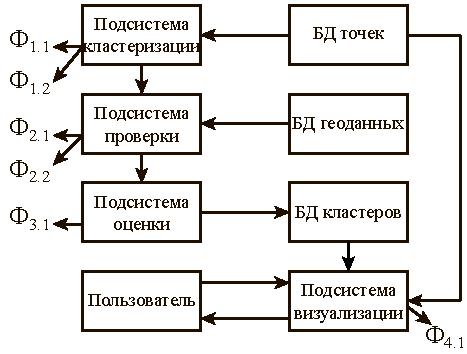
\includegraphics[width=.7\textwidth]{cfs}
  \caption{Конструктивно-функциональная структура в виде графа}
\end{figure}

\chapter{Потоково-функциональный анализ}

\begin{table}[h!]
  \centering
  \small
  \caption{Потоковая функциональная структура прототипа}
  \begin{tabular}{|C{.04}|C{.15}|C{.16}|C{.07}|C{.16}|C{.17}|C{.07}|} \hline
    \multirow{5}{.04\textwidth}{\centering Но\-мер} &
      \multirow{5}{.15\textwidth}{\centering Наимено\-вание элемента и
        объекта ОС} &
      \multicolumn{5}{c|}{Информационная операция} \\ \cline{3-7}
    & & Вход \( A_T \) & Номер <<источника>> & Операция преобразования входа в
      выход & Выход \( C_T \) & Номер <<приемника>> \\ \hline
    1 & 2 & 3 & 4 & 5 & 6 & 7 \\ \hline
    
    \multirow{2}{*}{1-1} &
      \multirow{2}{*}{БД точек} &
      & & & Точки (т) & 1 \\ \cline{3-7}
    & & & & & Точки (т) & 4 \\ \hline
    
    \multirow{3}{*}{1-2} &
      \multirow{3}{.15\textwidth}{\centering БД кластеров} &
      Сохранение информации о кластерах (ск) & 3 & & & \\ \cline{3-7}
    & & & & & Информация о кластерах (ик) & 4 \\ \hline
    
    1-3 & БД географических данных & & & & Геоданные (г) & 2 \\ \hline
    
    1 & Подсистема кластеризации &
      Точки (т) & 1-1 & Кластери\-зация & Информация о кластерах (ик) &
      2 \\ \hline
      
    2 & Подсистема проверки &
      Геоданные (г); Информация о кластерах (ик) & 1-3; 1 &
      Разбиение/ слияние кластеров & Информация о кластерах (ик) & 3 \\ \hline
      
    3 & Подсистема оценки &
      Информация о кластерах (ик) & 2 & Оценка &
      Сохранение информации о кластерах (ск) & 1-2 \\ \hline
    
    \multirow{4}{*}{4} &
      \multirow{4}{.15\textwidth}{\centering Подсистема визуализации} &
      Информация о кластерах (ик); точки (т) & 1-2; 1-1 &
      Отображение результата & Графический результат (гр) & 5 \\ \cline{3-7}
    & & Управляющее воздействие (ув) & 5 & Отображение результата &
      Графический результат (гр) & 5 \\ \hline
      
    \multirow{3}{*}{5} &
      \multirow{3}{*}{Пользователь} &
      & & & Управляющее воздействие (ув) & 4 \\ \cline{3-7}
    & & Графический результат (гр) & 4 & & & \\ \hline
  \end{tabular}
\end{table}

\newpage

\begin{figure}[h!]
  \center
  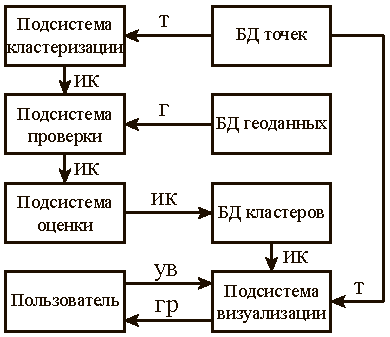
\includegraphics[width=.6\textwidth]{ffs} \\
  \caption{Потоковая функциональная структура}
\end{figure}

\chapter{Функционально-физический анализ прототипа, оценка целостности}
\emph{Конструктивно-функциональный анализ, операции Коллера}
\begin{table}[h!]
  \centering
  \small
  \caption{Конструктивно-функциональный анализ}
  \begin{tabular}{|*{2}{C{.08}|C{.18}|}C{.15}|C{.15}|} \hline
    \multicolumn{2}{|c|}{Элемент} & \multicolumn{4}{c|}{Преобразования}\\ \hline
    Обозна\-чение & Наименование & Обозна\-чение & Наименование &
      Операция Коллера & Обратная операция Коллера \\ \hline
    \multirow{4}{*}{\( E_1 \)} &
      \multirow{4}{.18\textwidth}{\centering Подсистема кластеризации} &
      \( \Phi_{1.1} \) & Настройка параметров кластеризации &
      Излучение & Поглощение \\ \cline{3-6}
    & &
      \( \Phi_{1.2} \) & Расчет центроидов &
      Преобра\-зование & Обратное преобра\-зование \\ \hline
    \multirow{4}{*}{\( E_2 \)} &
      \multirow{4}{.18\textwidth}{\centering Подсистема проверки} &
      \( \Phi_{2.1} \) & Поиск нужных точек &
      Преобра\-зование & Обратное преобра\-зование \\ \cline{3-6}
    & &
      \( \Phi_{2.2} \) & Разбиение и слияние кластеров &
      Преобра\-зование & Обратное преобра\-зование \\ \hline
    \( E_3 \) & Подсистема оценки &
      \( \Phi_{3.1} \) & Оценка кластеризации &
      Накопление & Выдача \\ \hline
    \( E_4 \) & Подсистема визуализации &
      \( \Phi_{4.1} \) & Отображение центроидов и точек &
      Отобра\-жение & Обратное отобра\-жение \\ \hline
  \end{tabular}
\end{table}

\newpage

\emph{Описание прототипа как информационной системы}
\begin{table}[h!]
  \centering
  \small
  \caption{Потоковая функциональная структура прототипа}
  \begin{tabular}{|C{.105}|*{4}{C{.18}|}} \hline
    \multirow{4}{.105\textwidth}{\centering
        Номер элемента и~объекта ОС} &
      \multirow{4}{.18\textwidth}{\centering
        Наименование элемента и объекта ОС} &
      \multicolumn{3}{c|}{Информационная операция} \\ \cline{3-5}
    & & Входное воздействие \( A \) на элемент &
      Операция Коллера &
      Выходное воздействие \( C \) элемента \\ \hline
    
    1-1 & БД точек & & Излучение & Точки (т) \\ \hline
    \multirow{3}{*}{1-2} & 
      \multirow{3}{*}{БД кластеров} &
      Сохранение информации о кластерах (ск) & Накопление & \\ \cline{3-5}
    & & &
      Излучение & Информация о кластерах (ик) \\ \hline
    1-3 & БД географических данных & & Излучение & Геоданные (г) \\ \hline
    1 & Подсистема кластеризации &
      Точки (т) & Преобразование & Информация о кластерах (ик) \\ \hline
    2 & Подсистема проверки &
      Геоданные (г); Информация о кластерах (ик) &
      Преобразование & Информация о кластерах (ик) \\ \hline
    3 & Подсистема оценки &
      Информация о кластерах (ик) &
      Накопление & Сохранение информации о кластерах (ск) \\ \hline
    \multirow{3}{*}{4} &
      \multirow{3}{.18\textwidth}{\centering Подсистема визуализации} &
      Информация о кластерах (ик); точки (т) &
      Отображение & Графический результат (гр) \\ \cline{3-5}
    & & Управляющее воздействие (ув) &
      Отображение & Графический результат (гр) \\ \hline
    \multirow{3}{*}{5} &
      \multirow{3}{*}{Пользователь} & &
      Преобразование & Управляющее воздействие (ув) \\ \cline{3-5}
    & & Графический результат (гр) & Преобразование & \\ \hline
  \end{tabular}
\end{table}

\emph{Диаграмма Исикавы}
\begin{figure}[h!]
  \center
  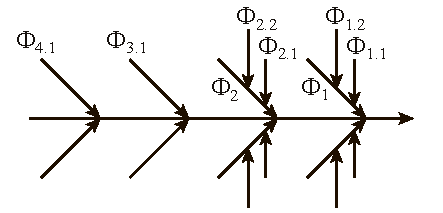
\includegraphics[width=.43\textwidth]{Ishikawa}
  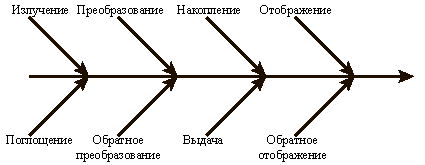
\includegraphics[width=.54\textwidth]{Ishikawa2}
  \caption{Диаграммы Исикавы для главной функции и для операций Колера
    (инвертированные функции снизу)}
\end{figure}

Целостность системы: \( 8 / 16 = 0.5 \).

\chapter{Синтез новых технических решений на основе использования
  эвристических приемов, оценка новизны решений}
  
\begin{table}[h!]
  \centering
  \small
  \caption{Синтез новых решений с использованием ЭП}
  \begin{tabular}{|C{.03}|*{4}{C{.2}|}} \hline
    № п/п & Формулировка ЭП & Интерпретация ЭП &
      Синтезированное решение с использованием ЭП &
      Устраняемый недостаток прототипа \\ \hline
    1 & Увеличить~эффективность~действия~путем~последовательного применения~%
      группы~однородных объектов (элементов) &
      Предусмотреть возможность задавать параметры кластеризации &
      Реализовать возможность выбора пользователем параметров кластеризации &
      Невозможность учитывать некоторые параметры при кластеризации \\ \hline
    2 & Увеличить степень дробления (измельчения) объекта. Инверсия~приема &
      Добавить возможность варьировать число кластеров &
      Реализовать функцию изменения числа кластеров &
      Неточности в расчетах центроидов \\ \hline
    3 & Присоединить новый ингредиент или заменить его  &
      Предусмотреть возможность выбора кластеров для слияния и разделения &
      Реализовать функциональную возможность выбора кластеров для слияния
      или разбиения &
      Некорректный выбор кластеров для слияния или разбиения \\ \hline
    4 & Увеличить~эффективность~действия~путем~последовательного применения~%
      группы~однородных объектов (элементов) &
      Использовать симметрию или асимметрию и изменение форм объектов в
      интерфейсе &
      Сделать~интерфейс~с~использованием~нестандартных~решений~для~повышения~%
      его~наглядности~и~простоты использования &
      Наглядность интерфейса \\ \hline
    5 & Ввести элементы, допускающие или обеспечивающие сборку объекта только
      в нужном положении &
      Задать возможность выбора качества (оценки) проделанной кластеризации &
      Реализовать несколько критериев оценки кластеризации на основе простых
      алгоритмов кластеризации &
      Оценка кластеризации \\ \hline
  \end{tabular}
\end{table}
  
\newpage

\begin{table}[h!]
  \centering
  \small
  \caption{Синтез новых решений с использованием инвертированных ЭП}
  \begin{tabular}{|C{.03}|C{.2}|*{4}{C{.15}|}} \hline
    № п/п & Формулировка ЭП & Инверсный ЭП & Интерпре\-тация~ЭП &
      Синтезиро\-ванное~решение~с~использованием~ЭП &
      Устраняемый недостаток прототипа \\ \hline
    1 & Преобразовать неподвижный объект (элемент) в подвижный;
      обеспечить~перемещение~элемента~в~объекте. Инверсия приема &
      Зафиксировать подвижный элемент &
      Задавать жесткий набор параметров &
      Реализовать возможность выбора пользователем параметров из
      заданного набора &
      Невозмож\-ность~учитывать~некоторые~параметры~при~кластеризации \\ \hline
    2 & Перейти от последовательного~осуществления~операций~к~параллельному~%
      (одновременному). Инверсия приема &
      Перейти от параллельного~осуществления~операций~к~последовательному &
      Объединять и разделять кластеры~на каждой~итерации~после расчетов
      центроидов &
      Реализовать алгоритм объединения и разделения кластеров для
      неконечных данных &
      Неточности в расчетах центроидов \\ \hline
    3 & Увеличить степень дробления (измельчения) объекта &
      Объединение элементов объекта &
      Предусмот\-реть~возможность выбора кластеров для слияния и разделения &
      Реализовать функциональную~возможность~выбора~кластеров~для~слияния~%
      или~разбиения &
      Некорректный выбор~кластеров~для~слияния~или~разбиения \\ \hline
    4 & Присоединить новый ингредиент или заменить его &
      Удалить один из существующих~ингредиентов &
      Упростить интерфейс &
      Убрать~лишние элементы из~интерфейса, упростить его &
      Наглядность интерфейса \\ \hline
    5 & Заменить объект (элемент) более простым &
      Заменить объект (элемент) более сложным &
      Задать возможность выбора~качества~(оценки)~проделанной~кластеризации &
      Реализовать несколько критериев оценки кластеризации на основе~%
      алгоритмов~кластеризации &
      Оценка кластеризации \\ \hline
  \end{tabular}
\end{table}

\newpage

\begin{table}[h!]
  \centering
  \small
  \caption{Сравнение прототипа и синтезированных решений}
  \begin{tabular}{|C{.1}|*{3}{C{.25}|}} \hline
    № п/п & Перечень~отличительных~признаков~прототипа &
      Перечень~отличительных~признаков~синтезированного~нового решения &
      Результат сравнения \\ \hline
    1 & Невозможность учитывать некоторые параметры при кластеризации &
      Интерфейс с возможностью задавать параметры кластеризации &
      Повышение качества кластеризации \\ \hline
    Новизна & \multicolumn{3}{C{.8}|}{
      Разработана новая система, отличающаяся от предыдущей включением в
      интерфейс возможности задавать параметры кластеризации, за счет чего
      повышается точность и качество кластеризации} \\ \hline
    2 & Неточные расчеты центроидов &
      Возможность варьировать число кластеров &
      Повышение качества кластеризации \\ \hline
    Новизна & \multicolumn{3}{C{.8}|}{
      Разработана новая система, отличающаяся от предыдущей включением
      возможности менять количество кластеров, за счет чего повышается
      точность и качество кластеризации} \\ \hline
    3 & Некорректный выбор кластеров для слияния или разбиения &
      Возможность выбора кластеров для слияния или разбиения &
      Повышение качества и эффективности кластеризации \\ \hline
    Новизна & \multicolumn{3}{C{.8}|}{
      Разработана новая система, отличающаяся от предыдущей возможностью
      выбирать кластеры, подлежащие слиянию или разбиению, за счет чего
      повышается качество кластеризации} \\ \hline
    4 & Отсутствие интуитивно понятного интерфейса &
      Интуитивно понятный интерфейс &
      Повышение удобства и простоты работы с системой \\ \hline
    Новизна & \multicolumn{3}{C{.8}|}{
      Разработана новая система, отличающаяся от предыдущей интерфейсом,
      измененным для повышения удобства и простоты работы с системой} \\ \hline
    5 & Невозможность оценки качества кластеризации &
      Возможность оценивать качество кластеризации &
      Повышение~наглядности, качества~работы~и эффективности работы
      программы \\ \hline
    Новизна & \multicolumn{3}{C{.8}|}{
      Разработана новая система, отличающаяся от предыдущей наличием базовых
      алгоритмов кластеризации, отталкиваясь от результатов которых можно по
      определенным параметрам оценивать проделанную системой
      кластеризацию} \\ \hline
  \end{tabular}
\end{table}
  
\chapter{Постановка задачи поиска нового технического решения с
  описанием синтезированных решений и оценкой их новизны}
Решение 1.
\begin{enumerate}
  \item \emph{Недостаток}~-- недостаточная наглядность интерфейса.
  \item Подсистема визуализации.
  \item Экранная форма.
  \item \emph{Изменение параметра}:
    \begin{itemize}
      \item отрисовка результатов кластеризации;
      \item выбор параметров кластеризации.
    \end{itemize}
  \item \emph{Конфликт между показателями качества}: П1~-- наглядность работы
    системы, П2~-- загруженность интерфейса. Повышение наглядности работы
    системы приводит к перегруженности интерфейса.
  \item \emph{Функциональный конфликт}: Ф1~-- функция наглядности работы
    системы, Ф2~-- функция загруженности.
  \item \emph{Конфликт свойств}: С1~-- интерфейс должен поддерживать
    возможность изменения параметров кластеризации, С2~-- интерфейс не должен
    поддерживать возможность изменения параметров кластеризации.
  \item \emph{Изменение системы}. Заменить узловой элемент объектом, который на
    различных фазах жизненного цикла исходной системы характеризуется
    различными значениями параметра, указанного в формуле конфликта свойств.
  \item \emph{Решение}. Скрыть неиспользуемые элементы интерфейса от
    пользователя.
\end{enumerate}

\newpage

Решение 2.
\begin{enumerate}
  \item \emph{Недостаток}~-- некорректный выбор кластеров для слияния или
    разбиения.
  \item Подсистема проверки.
  \item Момент времени проверки.
  \item \emph{Изменение параметра}:
    \begin{itemize}
      \item возможность вручную задавать кластеры для слияния или разбиения.
    \end{itemize}
  \item \emph{Конфликт между показателями качества}: П1~-- точность
    кластеризации, П2~-- время кластеризации. Повышение точности кластеризации
    приводит к увеличению времени кластеризации.
  \item \emph{Функциональный конфликт}: Ф1~-- функция точности кластеризации,
    Ф2~-- функция времени кластеризации.
  \item \emph{Конфликт свойств}: С1~-- подсистема должна поддерживать
    возможность задания кластеров вручную, С2~-- подсистема не должна
    поддерживать возможность задания кластеров вручную.
  \item \emph{Изменение системы}. Выполнить вспомогательные действия или часть
    основного действия до или после основного действия.
  \item \emph{Решение}. Реализовать возможность задавать набор конкретных
    кластеров для разбиения или слияния до начала кластеризации, не прерывая
    работу системы. Импорт параметров из файла конфигурации.
\end{enumerate}

\newpage

Синтезировать новые решения с помощью процедур постановки задачи поиска нового
технического решения для реализации инверсных операций Коллера по результатам
конструктивно-функционального анализа:

Решение 3.\\
\emph{Элемент}~-- подсистема кластеризации.\\
\emph{Операция Коллера}~-- преобразование.\\
\emph{Инверсная операция Коллера}~-- обратное преобразование.\\
Реализовать возможность изменения параметров кластеризации для повышения
качества кластеризации.\\

Решение 4.\\
\emph{Элемент}~-- подсистема оценки.\\
\emph{Операция Коллера}~-- преобразование.\\
\emph{Инверсная операция Коллера}~-- обратное преобразование.\\
Реализовать возможность оценки качества кластеризации путем сравнения с
алгоритмами с известной оценкой из стандартного набора.\\

Решение 5.\\
\emph{Элемент}~-- подсистема визуализации.\\
\emph{Операция Коллера}~-- отображение.\\
\emph{Инверсная операция Коллера}~-- обратное отображение.\\
Реализовать возможность вывода оценки качества кластеризации.

\newpage

Оценить новизну полученных решений на основе сравнения отличительных признаков
прототипа и нового решения.

В результате работы синтезировано 5 новых решений.
\begin{table}[h!]
  \centering
  \small
  \caption{Сравнение прототипа и синтезированных решений}
  \begin{tabular}{|C{.1}|*{3}{C{.25}|}} \hline
    № п/п & Перечень~отличительных~признаков~прототипа &
      Перечень~отличительных~признаков~синтезированного~нового решения &
      Результат сравнения \\ \hline
    1 & Недостаточная наглядность интерфейса &
      Наглядный и удобный интерфейс &
      Повышение удобства и простоты работы с системой \\ \hline
    Новизна & \multicolumn{3}{C{.8}|}{
      Разработана новая система, отличающаяся от предыдущей тем, что с ней
      удобней и проще работать: настройки параметров могут быть скрыты от
      пользователя при желании}
      \\ \hline
    2 & Объединяемые~и~разделяемые~кластеры~выбираются~некорректно &
      Корректный выбор кластеров &
      Повышение качества кластеризации \\ \hline
    Новизна & \multicolumn{3}{C{.8}|}{
      Разработана новая система, отличающаяся от предыдущей наличием выбора
      кластеров для слияния и разбиения, что повышает точность и качество
      кластеризации} \\ \hline
    3 & Ненастраиваемые параметры кластеризации &
      Перечень~настраиваемых~параметров~кластеризации &
      Повышение качества кластеризации \\ \hline
    Новизна & \multicolumn{3}{C{.8}|}{
      Разработана новая система, отличающаяся от предыдущей наличием списка
      настраиваемых параметров кластеризации, что повышает ее качество}
      \\ \hline
    4 & Нет сравнительной оценки качества &
      Наличие параметров, оцененных на стандартных примерах &
      Повышение качества кластеризации \\ \hline
    Новизна & \multicolumn{3}{C{.8}|}{
      Разработана новая система, отличающаяся от предыдущей наличием
      сравнительной оценки проведенной кластеризации, что позволяет выбрать
      наилучший алгоритм для дальнейшего использования} \\ \hline
    5 & Нет вывода оценки качества &
      Реализован вывод оценки &
      Повышение наглядности работы системы \\ \hline
    Новизна & \multicolumn{3}{C{.8}|}{
      Разработана новая система, отличающаяся от предыдущей включением показа
      оценки проведенной кластеризации для пользователя для большей наглядности
      и удобства работы} \\ \hline
  \end{tabular}
\end{table}

\chapter{Синтез заставки}
1. Гирлянда синонимов к слову кластер: группа, класс, свойство, объединение.

2. Случайные объекты: яблоко, стол, перо, ключ.

3. Составление комбинаций из элементов гирлянды синонимов объекта и элементов
гирлянды случайных объектов:\\
группа яблок, групповой стол, группа перьев, групповой ключ, классное яблоко,
классное дерево, классное перо, классный ключ, свойственное яблоко,
свойственный стол, свойственное перо, свойственный ключ, объединенное яблоко,
объединенный стол, объединенное перо, объединенный ключ, яблочная группа,
столовая группа, перьевая группа, ключевая группа, яблочный класс,
столовый класс, перьевой класс, ключевой класс, яблочное свойство,
столовое свойство, перьевое свойство, ключевое свойство, яблочное объединение,
столовое объединение, перьевое объединение, ключевое объединение.

4. Составление признаков случайных объектов:
\begin{table}[h!]
    \centering
    \small
    \begin{tabular}{|C{.15}|C{.6}|} \hline
        Объект & Признаки \\ \hline
        яблоко & зеленое, сочное, круглое \\ \hline
        стол   & деревянный, квадратный, обеденный \\ \hline
        перо   & мягкое, черное, письменное \\ \hline
        ключ   & старинный, серебряный, дверной \\ \hline
    \end{tabular}
\end{table}

5. Генерирование идей путем поочередного присоединения к техническому объекту и
его синонимам признаков случайно выбранных объектов:
\begin{table}[h!]
  \centering
  \small
  \begin{tabular}{|C{.1}|C{.8}|} \hline
    Группа & зеленая группа, сочная группа, круглая группа, деревянная группа,
      квадратная группа, обеденная группа, мягкая группа, черная группа,
      письменная группа, старинная группа, серебряная группа, дверная группа
      \\ \hline
    Класс & зеленый класс, сочный класс, круглый класс, деревянный класс,
      квадратный класс, обеденный класс, мягкий класс, черный класс,
      письменный класс, старинный класс, серебряный класс, дверной класс
      \\ \hline
    Свойство & зеленое свойство, сочное свойство, круглое свойство,
      деревянное свойство, квадратное свойство, обеденное свойство,
      мягкое свойство, черное свойство, письменное свойство,
      старинное свойство, серебряное свойство, дверное свойство
      \\ \hline
    Объедине\-ние & зеленое объединение, сочное объединение,
      круглое объединение, деревянное объединение, квадратное объединение,
      обеденное объединение, мягкое объединение, черное объединение,
      письменное объединение, старинное объединение, серебряное объединение,
      дверное объединение
      \\ \hline
    \end{tabular}
\end{table}

\newpage

6. Генерирование гирлянд ассоциаций:
\begin{table}[h!]
    \centering
    \small
    \begin{tabular}{|C{.15}|C{.6}|} \hline
        зеленый & луг, трава, краска \\ \hline
        сочный  & персик, помидор, цвет \\ \hline 
        круглый & блин, шар, неудачник \\ \hline
        деревянный & табурет, рубль, игрушка \\ \hline
        квадратный & ковер, проход, монитор \\ \hline
        обеденный & зал, комната, час \\ \hline
        мягкий & диван, подушка, пуховик \\ \hline
        черный & туча, дыра, волос \\ \hline
        письменный & стол, принадлежность, речь \\ \hline
        старинный & сундук, з\'{а}мок, артефакт \\ \hline
        серебряный & ложка, слиток, кубок \\ \hline
        дверной & зам\'{о}к, ручка, глазок \\ \hline
    \end{tabular}
\end{table}

7. Генерирование новых идей: зеленый луг, сочный круглый блин,
черный деревянный ковер, старинный дверной зам\'{о}к, старинная серебряная
ложка, черная письменная ручка, мягкий сочный глазок, квадратный старинный
диван, мягкий зеленый слиток, круглая старинная игрушка, обеденный сочный
табурет, старинная дверная ручка, старинный обеденный кубок, черный круглый
монитор, мягкий черный цвет, сочный зеленый помидор, мягкий квадратный пуховик,
черный старинный з\'{а}мок, сочная трава, квадратная обеденная комната.

8. Выбор рациональных вариантов: черный старинный з\'{а}мок, старинный
обеденный кубок, зеленый луг, сочная трава, квадратная обеденная комната.

9. Окончательный синтез заставки. \\
На зеленом лугу покрытом сочной травой возвышался старинный черный замок. Люди
входят внутрь и попадают в квадратную обеденную комнату, посреди которой стоит
деревянный стол, накрытый к пиршеству -- на нем стоят различные серебряные кубки
и столовые приборы, однако, весь стол покрыт толстым слоем пыли.

\chapter{Выводы}
В ходе выполнения работы были реализованы различные методы создания технических
решений для метода кластеризации предпочтений жителей города по перемещению.
Реализованы следующие этапы синтеза новых технических решений:
\begin{enumerate}
  \item Конструктивно-функциональный анализ прототипа. На этом этапе система
    декомпозируется на элементы, описываются функции элемента и приводится
    оценка этих функций (конструктивно-функциональная структура прототипа). Это
    необходимо для определения недостатков прототипа и постановки целей
    совершенствования системы. Далее приводится потоковая структура
    прототипа для описания информационных процессов, происходящих в системе.
    Приводится конструктивно-функциональная структура в виде графа, на которой
    отображаются элементы системы и их функции.
  \item Функционально-информационный анализ прототипа. Этот этап необходим для
    определения операций Коллера, описания прототипа как информационной
    системы. 
  \item Построение диаграмм Исикавы по функционалу прототипа, определение
    целостности системы. Этот этап необходим для выявления взаимосвязей между
    различными функциями системы, понимания существенных факторов, которые
    влияют на работу системы, более глубокого понимания недостатков системы.
    В результате построения диаграммы Исикавы по функционалу прототипа были
    установлены цели совершенствования технической системы, а также был
    произведен расчет целостности системы, который составляет 0.5.
  \item Синтез новых решений по совершенствованию прототипа. Проведен синтез
    решений с использованием эвристических приемов и инвертированных
    эвристических приемов. В результате этого этапа было синтезировано 5 новых
    решений, которые позволяют повысить эффективность системы.
    Первое решение отличается от прототипа переработкой интерфейса и
    возможностью скрыть настройки параметров, за счет чего повышается
    эффективность работы с системой.
    Второе решение отличается от прототипа включением в него возможности
    выбора кластеров для слияния и разбиения, что повышает точность и качество
    кластеризации.
    Третье решение отличается от прототипа тем, что в систему добавлен список
    настраиваемых параметров кластеризации, за счет чего повышается качество
    работы программы.
    Четвертое решение отличается от прототипа тем, что в нем добавлена
    возможность использовать сравнение для оценки проведенной кластеризации,
    что позволяет выбрать наилучший алгоритм для дальнейшего использования.
    Пятое решение отличается от прототипа тем, что в интерфейс включен показ
    оценки проведенной кластеризации пользователю для большей наглядности и
    удобства работы.
  \item Постановка задачи поиска нового решения. На этом этапе поставлена
    задача поиска нового решения с описанием новых синтезированных решений и
    оценкой новизны. Предложены решения по реализации инверсных операций
    Коллера. Лучшими решениями на данном этапе являются решения:
    решение с возможностью задавать жесткий набор параметров (повышение
    точности кластеризации), решение с объединением и разделением кластеров
    после каждой итерации расчетов центроидов (повышение качества
    кластеризации), решение с возможностью мануального выбора кластеров для
    слияния и разделения (повышение качества кластеризации), решение с сильно
    упрощенным интерфейсом (повышение удобства работы с программой), решение с
    возможностью оценки качества кластеризации (повышение качества
    кластеризации).
    
    Таким образом, лучшее решение заключается в разработке системы с более
    наглядным интерфейсом, возможностью оценивать кластеризацию и мануально
    задавать кластеры для слияния и разделения, а также изменять параметры
    кластеризации. Синтезированное решение повышает удобство работы с системой,
    точность и качество ее работы.
  \item Разработана заставка, которая отображается при установке системы. 
    На зеленом лугу покрытом сочной травой возвышался старинный черный замок.
    Люди входят внутрь и попадают в квадратную обеденную комнату, посреди
    которой стоит деревянный стол, накрытый к пиршеству~-- на нем стоят
    различные серебряные кубки и столовые приборы, однако, весь стол покрыт
    толстым слоем пыли.
\end{enumerate}